\documentclass[11pt,a4paper]{article}
\usepackage[margin=1in]{geometry}
\usepackage[T1]{fontenc}
\usepackage{lmodern}
\usepackage{microtype}
\usepackage{amsmath}
\usepackage{xcolor}
\definecolor{kthblue}{HTML}{004791}
\usepackage[hyphens,spaces,obeyspaces]{xurl}
\usepackage{booktabs}
\usepackage{tabularx}
\usepackage{array}
\usepackage{needspace}
\usepackage{float}
\usepackage{enumitem}
\usepackage{graphicx}
\usepackage{fancyhdr}
\usepackage{parskip}
\usepackage{hyperref}

\newcolumntype{Y}{>{\raggedright\arraybackslash}X}
\emergencystretch=2em
\setlength{\tabcolsep}{5pt}
\renewcommand{\arraystretch}{1.18}
\renewcommand{\contentsname}{}
\newcommand{\tocentry}[1]{\addcontentsline{toc}{section}{#1}}

\hypersetup{
    colorlinks=true,
    linkcolor=kthblue,
    urlcolor=kthblue,
    pdftitle={Applied GPU Programming -- Assignment 1},
    pdfauthor={Group 40: Yuanyu Zhang, Hongen Wang, Xinyang Li},
}
\title{Applied GPU Programming -- Assignment 1}
\author{Group 40 -- Yuanyu Zhang, Hongen Wang, Xinyang Li}
\date{6 November 2026}

\pagestyle{fancy}
\fancyhf{}
\fancyhead[L]{\small Applied GPU Programming -- Group 40}
\fancyhead[R]{\small Assignment 1}
\fancyfoot[C]{\small \thepage}
\renewcommand{\headrulewidth}{0.4pt}
\setlength{\headheight}{14pt}

\begin{document}

\pagenumbering{gobble}
\hypersetup{pageanchor=false}
\begin{titlepage}
\thispagestyle{empty}
\centering
\vspace*{1.0cm}

\begingroup
\setlength{\fboxsep}{12pt}
\colorbox{kthblue}{
\includegraphics[height=2.8cm]{kth-logo.png}}
\endgroup

\vspace{0.35cm}
{\footnotesize KTH Electrical Engineering and Computer Science}

\vspace{1.6cm}

{\LARGE\bfseries Assignment 1\\[0.45cm]
CUDA Vector Addition and Matrix Multiplication\\[0.25cm]
and Quantum Fourier Transform Profiling}

\vspace{1.2cm}

{\small Applied GPU Programming \textperiodcentered\ HT26}

\vfill

{\large Group 40}\\[0.55cm]
{\normalsize Yuanyu Zhang \textperiodcentered\ Hongen Wang \textperiodcentered\ Xinyang Li}

\vspace{1.4cm}

{\small Stockholm, 6 November 2026}
\vspace*{0.3cm}
\end{titlepage}
\hypersetup{pageanchor=true}
\pagenumbering{arabic}

\tableofcontents
\vspace{1.5em}

\section*{Experimental environments}
\tocentry{Experimental environments}
\begin{table}[H]
\centering
\begin{tabularx}{\textwidth}{@{}lYYY@{}}
\toprule
\textbf{Question} & \textbf{GPU and system} & \textbf{CUDA and profiler} & \textbf{Purpose} \\
\midrule
Q1 & Tesla T4, Google Colab & CUDA 13.0.88, Nsight Compute 2025.3.1 & Timing, correctness and occupancy \\
Q2 & Tesla T4, Google Colab & CUDA 13.0.88, Nsight Compute 2025.3.1 & Timing, correctness and occupancy \\
Q3 & Tesla T4, Google Colab & QuEST CUDA backend, Nsight Systems & QFT runtime and memory profiling \\
\bottomrule
\end{tabularx}
\end{table}

All three questions use an NVIDIA T4 with compute capability 7.5. All Q2 timings are ordinary runs without profiler instrumentation. Each Q1/Q2 program runs one kernel per data point, without averaging repeated measurements.

\clearpage
\section*{Question 1 --- Your First CUDA Program and GPU Performance Metrics}
\tocentry{Question 1 --- CUDA Vector Addition}

\subsection*{1. Floating-point operations and global-memory reads}
For a vector of length \(N\), the kernel launches enough threads for one thread per element. Each valid thread performs one floating-point addition and reads one \texttt{float} from each input vector. Therefore,
\[
\text{FLOPs}=N, \qquad \text{global-memory reads}=2N.
\]
The kernel also performs \(N\) global-memory writes to the output vector.

\subsection*{2--3. Configuration and occupancy for \(N=512\)}
The block size is 32 threads. For \(N=512\), the launch uses \(512/32=16\) blocks, hence 512 threads in total. Nsight Compute reports 3.12\% achieved occupancy.

\subsection*{4. Correctness for \(N=263149\)}
The program works correctly. The grid size is rounded up with
\(\lceil N/32\rceil\), and the kernel guard \texttt{if (i < N)} prevents threads beyond the vector end from accessing memory. The maximum absolute CPU/GPU error is zero.

\subsection*{5--6. Configuration and occupancy for \(N=263149\)}
This launch uses 8,224 blocks and \(8{,}224\times32=263{,}168\) threads. Of these, 263,149 compute an output and 19 are inactive padding threads. The measured achieved occupancy is 33.67\%.

\begin{table}[H]
\centering
\begin{tabular}{@{}rrrrrr@{}}
\toprule
\(N\) & Blocks & Threads/block & Launched threads & Active threads & Achieved occupancy \\
\midrule
512 & 16 & 32 & 512 & 512 & 3.12\% \\
263,149 & 8,224 & 32 & 263,168 & 263,149 & 33.67\% \\
\bottomrule
\end{tabular}
\caption{Launch configurations and Nsight Compute achieved occupancy.}
\end{table}

\subsection*{7. Timing breakdown for increasing vector lengths}
Figure~\ref{fig:q1-timing} shows 16 lengths from 512 to 16,777,216, including \(N=263149\). Host-to-device time covers both inputs; device-to-host time covers one output. The two copies grow approximately linearly with \(N\) and dominate at large sizes, while the simple addition kernel remains a small fraction of total time.

\begin{figure}[H]
\centering
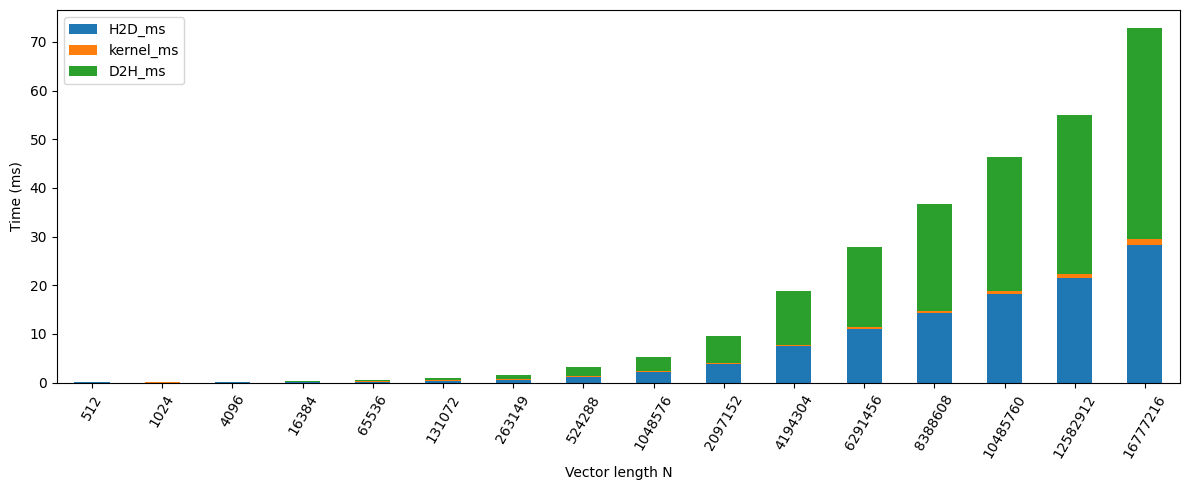
\includegraphics[width=\textwidth]{Q1/timing_breakdown.png}
\caption{Q1 timing breakdown on the Tesla T4.}
\label{fig:q1-timing}
\end{figure}

\subsection*{8. CPU/GPU numerical comparison}
The outputs match exactly for all tested lengths: \texttt{max\_error = 0}. Each result element is a single addition of the same two \texttt{float} operands on CPU and GPU, with no operation reordering or accumulated reduction error. Both therefore apply the same IEEE-754 rounding to the same exact sum. This does not imply that floating-point addition is exact in general; it means both implementations round identically here.

\clearpage
\section*{Question 2 --- 2D Dense Matrix Multiplication}
\tocentry{Question 2 --- 2D Dense Matrix Multiplication}

The program computes row-major \(C(M\times P)=A(M\times N)B(N\times P)\). Each valid thread computes one output element. Blocks contain \(16\times16=256\) threads, and the two-dimensional grid is
\[
\text{grid}=(\lceil P/16\rceil,\ \lceil M/16\rceil).
\]
The kernel uses no shared-memory tiling. The same templated implementation supports \texttt{double} and \texttt{float}.

\subsection*{1. Floating-point operations and global-memory reads}
Each of the \(MP\) output elements requires \(N\) multiplications and \(N\) additions to accumulate the dot product from an initial zero. Thus,
\[
\boxed{\text{FLOPs}=2MNP}.
\]
Each loop iteration reads one element of \(A\) and one element of \(B\), so the kernel performs
\[
\boxed{\text{global-memory reads}=2MNP}
\]
scalar element reads, or \(2MNP\,\text{sizeof}(T)\) bytes before considering cache effects. It also writes \(MP\) output elements. These are source-level global accesses; hardware caches can reduce actual DRAM traffic.

\subsection*{2. Small matrices: \(128\times256\) times \(256\times32\)}
The grid is \((\lceil32/16\rceil,\lceil128/16\rceil)=(2,8)\), giving 16 blocks and \(16\times256=4{,}096\) launched threads. Every thread computes one result because \(128\times32=4{,}096\). Nsight Compute reports \textbf{24.92\% achieved occupancy} (7.97 achieved active warps per SM; theoretical occupancy 100\%).

\subsection*{3. Large matrices: \(1024\times8191\) times \(8191\times8197\)}
The program still works. Two-dimensional launch bounds checks prevent out-of-range accesses, and 64-bit \texttt{size\_t} allocation/index arithmetic avoids 32-bit byte-size overflow. The double run passed 81 deterministic CPU-reference samples with zero maximum absolute error.

The grid is \((513,64)\), so there are \(513\times64=32{,}832\) blocks and \(32{,}832\times256=8{,}404{,}992\) launched threads. Only \(MP=1024\times8197=8{,}393{,}728\) threads compute results; the remaining 11,264 threads are padding in edge blocks. Nsight Compute reports \textbf{99.17\% achieved occupancy} (31.74 achieved active warps per SM). The much larger launch keeps the SMs occupied, unlike the 16-block small case.

\begin{table}[H]
\centering
\small
\begin{tabular}{@{}lrrrrr@{}}
\toprule
\((M,N,P)\) & Grid & Blocks & Launched threads & Active threads & Achieved occ. \\
\midrule
\((128,256,32)\) & \((2,8)\) & 16 & 4,096 & 4,096 & 24.92\% \\
\((1024,8191,8197)\) & \((513,64)\) & 32,832 & 8,404,992 & 8,393,728 & 99.17\% \\
\bottomrule
\end{tabular}
\caption{Q2 launch configurations and Nsight Compute achieved occupancy on the T4.}
\label{tab:q2-launch}
\end{table}

\subsection*{4. Timing breakdown with increasing matrix sizes}
Figure~\ref{fig:q2-double} shows the \texttt{double} timings. For the cubic cases, copy sizes grow approximately as the square of the side length, whereas kernel work grows as its cube. Copy and launch overheads are visible for small matrices; from \(1024^3\) onward the kernel is the largest component and its share increases rapidly. The naive inner loop repeatedly reads global memory and has no explicit data reuse through shared memory, which further increases kernel time.

\begin{figure}[H]
\centering
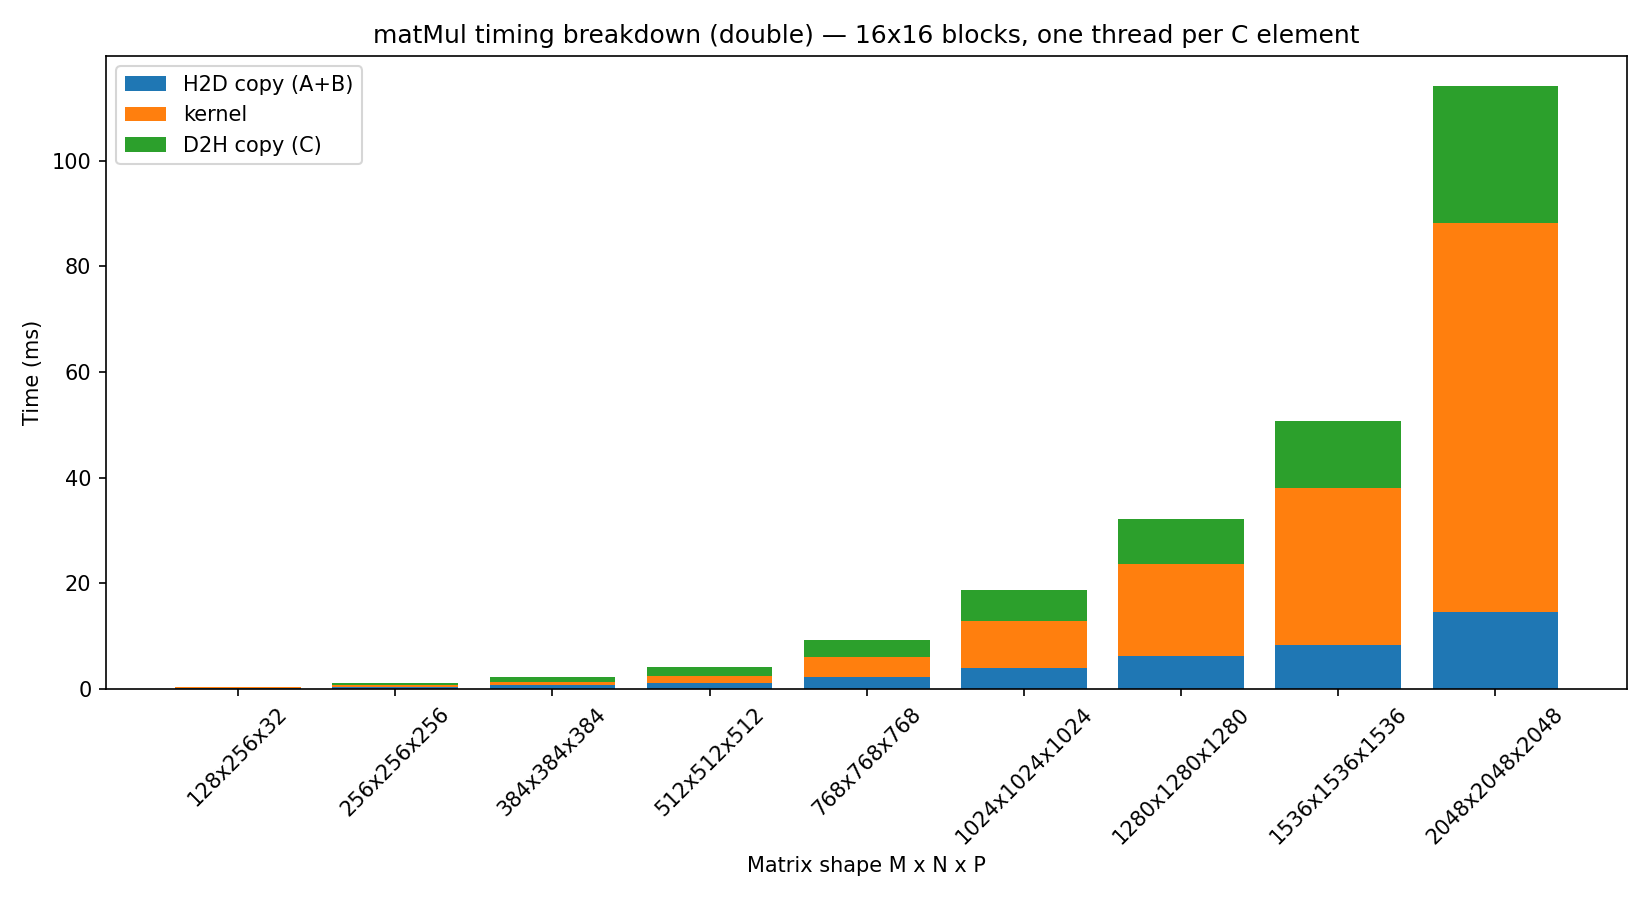
\includegraphics[width=\textwidth]{Q2/results/timing_double.png}
\caption{Q2 \texttt{double} timing breakdown on the Tesla T4.}
\label{fig:q2-double}
\end{figure}

\subsection*{5. Change from \texttt{double} to \texttt{float}}
Figure~\ref{fig:q2-float} repeats the same sweep with \texttt{float}. At \(2048^3\), H2D time falls from 14.6677 to 7.8645 ms (\(1.87\times\)) and D2H time from 25.9308 to 13.4261 ms (\(1.93\times\)), close to the ideal halving of transfer time because each element is half as large. Kernel time falls from 73.4890 to 31.2176 ms, a larger \(2.35\times\) speedup. Both reduced memory traffic and the T4's much higher FP32 than FP64 arithmetic throughput contribute. Total measured time falls from 114.0875 to 52.5082 ms (\(2.17\times\)). Smaller cases do not show the same ratio consistently because fixed launch and synchronization costs are significant.

\begin{figure}[H]
\centering
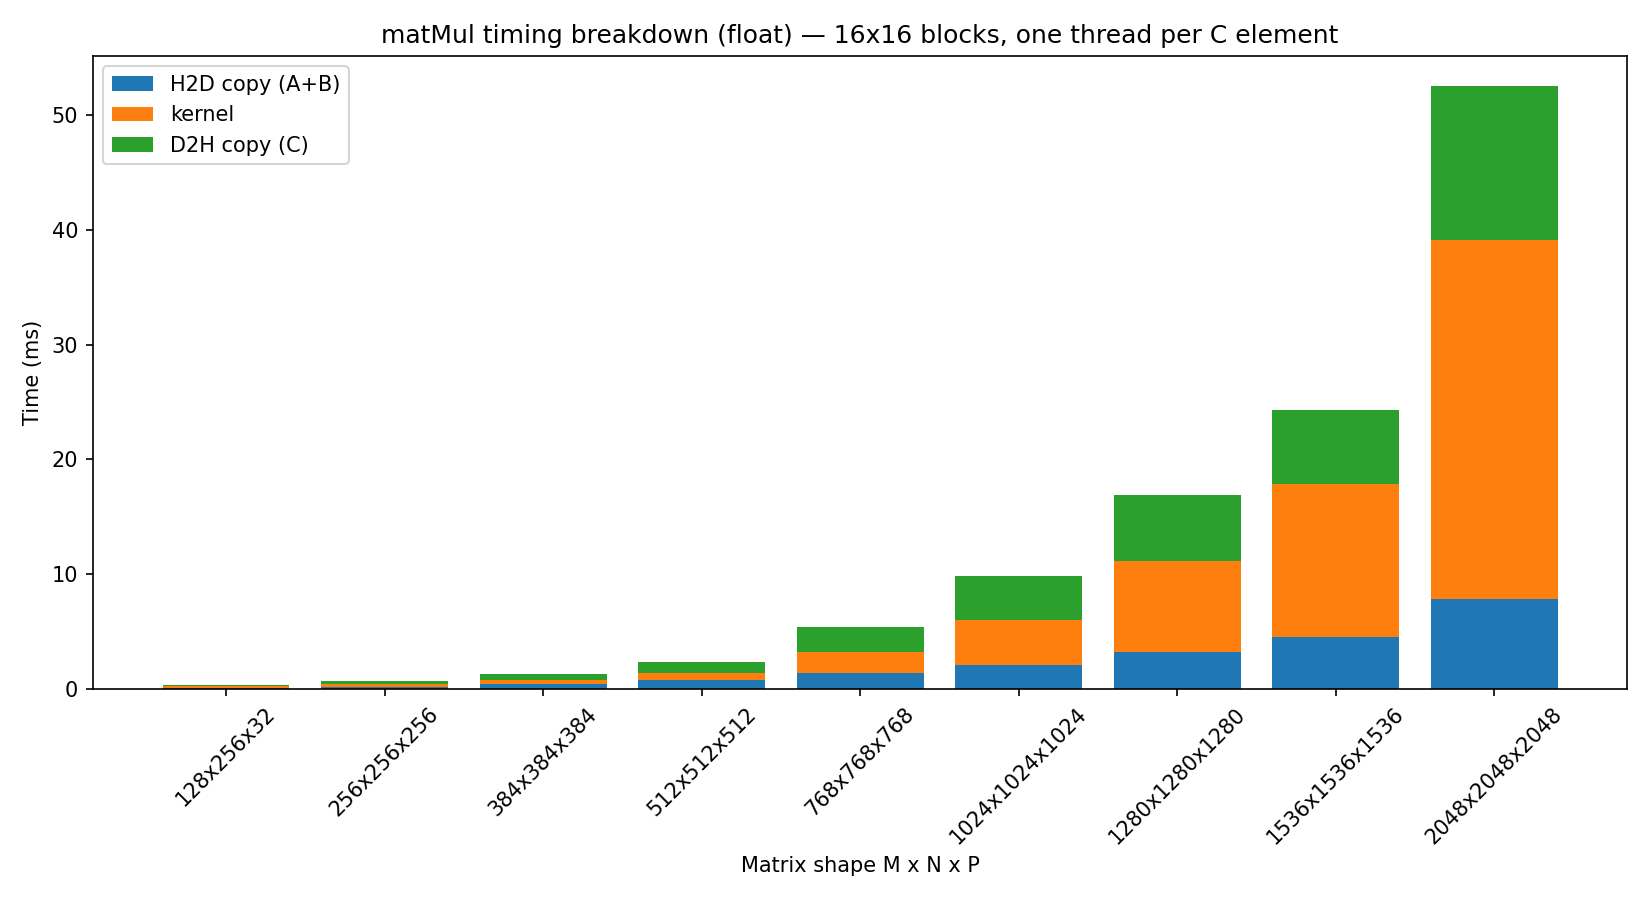
\includegraphics[width=\textwidth]{Q2/results/timing_float.png}
\caption{Q2 \texttt{float} timing breakdown on the Tesla T4.}
\label{fig:q2-float}
\end{figure}


\clearpage
\section*{Question 3 --- Quantum Fourier Transformation}
\tocentry{Question 3 --- Quantum Fourier Transformation}

\subsection*{3.1 Troubleshooting and 24-qubit run}
No troubleshooting was needed. The build commands from the assignment worked as given with compute capability 75, and the benchmark ran on the GPU backend.

\begin{figure}[H]
\centering
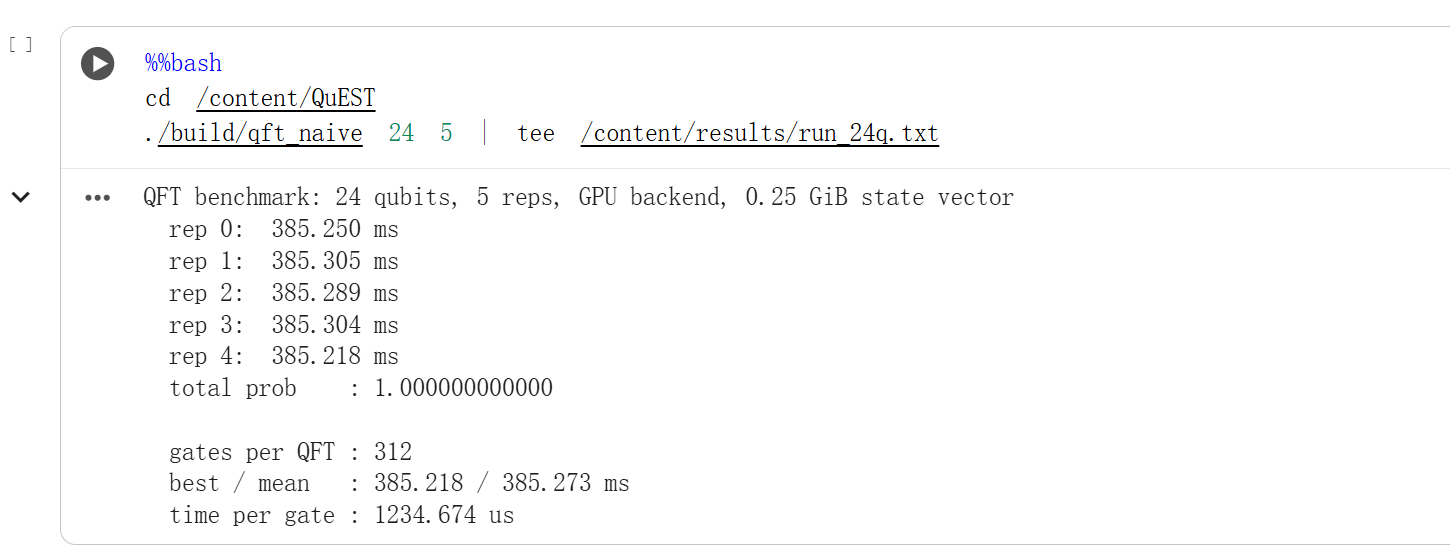
\includegraphics[width=\textwidth]{Q3/assets/image1.png}
\caption{Output of the 24-qubit QFT benchmark.}
\end{figure}

\subsection*{3.2 Memory at 28 qubits}
\begin{table}[H]
\centering
\begin{tabularx}{\textwidth}{@{}YYl@{}}
\toprule
\textbf{Quantity} & \textbf{Value} & \textbf{How obtained} \\
\midrule
GPU memory (whole device) & 4,203 MiB & \texttt{nvidia-smi memory.used}, polled during the run \\
GPU memory (this process) & 4,200 MiB & \texttt{nvidia-smi} per-process \texttt{used\_memory} \\
Process resident memory & 179 MiB & \texttt{/usr/bin/time -v} and \texttt{VmHWM} in \texttt{/proc/PID/status} \\
System memory in use & 1,308 MiB before; 1,515 MiB peak & \texttt{free -m} \\
\bottomrule
\end{tabularx}
\caption{Measured memory use for the 28-qubit benchmark.}
\end{table}

The run uses about 4.1 GiB of GPU memory. Almost all of it is the state vector: \(2^{28}\) amplitudes at 16 bytes each equal 4,096 MiB. System memory use is small, about 180 MiB for the process.

\subsection*{3.3 Top three kernels at 24 qubits}
The profile used the assignment's \texttt{nsys} command with \texttt{--trace=cuda,osrt --stats=true}, output prefix \texttt{qft\_24q}, and benchmark arguments \texttt{24 5}.

\begin{table}[H]
\centering
\small
\begin{tabularx}{\textwidth}{@{}rYrrrr@{}}
\toprule
\textbf{Rank} & \textbf{Kernel} & \textbf{Total (ms)} & \textbf{Time} & \textbf{Instances} & \textbf{Avg. (ms)} \\
\midrule
1 & \path{kernel_statevec_anyCtrlOneTargDiagMatr_sub<1>} & 1,874.1 & 80.8\% & 1,656 & 1.132 \\
2 & \path{kernel_statevec_anyCtrlOneTargDenseMatr_subA<0>} & 332.7 & 14.3\% & 144 & 2.311 \\
3 & \path{kernel_statevec_anyCtrlSwap_subA<0>} & 96.4 & 4.2\% & 72 & 1.338 \\
\bottomrule
\end{tabularx}
\caption{Nsight Systems GPU kernel summary for 24 qubits.}
\label{tab:q3-kernels}
\end{table}

The run has one warm-up and five timed QFTs, so each gate runs six times.

\subsection*{3.4 Kernels and quantum gates}
\begin{table}[H]
\centering
\small
\begin{tabularx}{\textwidth}{@{}YYr@{}}
\toprule
\textbf{Kernel} & \textbf{Gate} & \textbf{Per QFT (24 qubits)} \\
\midrule
\path{kernel_statevec_anyCtrlOneTargDiagMatr_sub} & \texttt{applyTwoQubitPhaseShift} & 276 \\
\path{kernel_statevec_anyCtrlOneTargDenseMatr_subA} & \texttt{applyHadamard} & 24 \\
\path{kernel_statevec_anyCtrlSwap_subA} & \texttt{applySwap} & 12 \\
\bottomrule
\end{tabularx}
\caption{Mapping from QuEST CUDA kernels to QFT gates.}
\end{table}

The phase gate is applied as a one-control, one-target diagonal matrix, the Hadamard as a dense \(2\times2\) matrix, and the swap through \texttt{localiser\_statevec\_anyCtrlSwap}. The kernels are in \texttt{quest/src/gpu/gpu\_kernels.cuh}. Six runs times 276, 24 and 12 give the instance counts in Table~\ref{tab:q3-kernels}. The phase kernel dominates total time because it runs 276 times per QFT.

\subsection*{3.5 CUDA API calls on the CPU thread}
A single CPU thread launches the kernels with \texttt{cudaLaunchKernel}, once per gate (312 per QFT). All 312 launches finish within 7.6 ms. The GPU needs 385 ms, so the CPU then waits in \texttt{cudaDeviceSynchronize}, which \texttt{syncQuESTEnv} calls.

\subsection*{3.6 Sixteen and 28 qubits}
\begin{table}[H]
\centering
\small
\begin{tabularx}{\textwidth}{@{}rYY@{}}
\toprule
\textbf{Qubits} & \textbf{QFT time, best / mean (ms)} & \textbf{Typical kernel: phase / Hadamard / swap} \\
\midrule
16 & 1.732 / 1.800 & 9.4 \(\mu\)s / 18.5 \(\mu\)s / 5.4 \(\mu\)s \\
24 & 384.96 / 385.00 & 1.13 ms / 2.31 ms / 1.18 ms \\
28 & 8,187.2 / 8,193.6 & 18.0 ms / 36.9 ms / 18.6 ms \\
\bottomrule
\end{tabularx}
\caption{QFT benchmark times and typical kernel durations.}
\end{table}

Kernel time scales with the state vector from 24 to 28 qubits: the state vector is 16 times larger and the kernels are about 16 times slower. At 16 qubits, kernels last only microseconds, similar to the approximately 5 \(\mu\)s launch cost, and the GPU is idle for about 15\% of a QFT.

\begin{figure}[H]
\centering
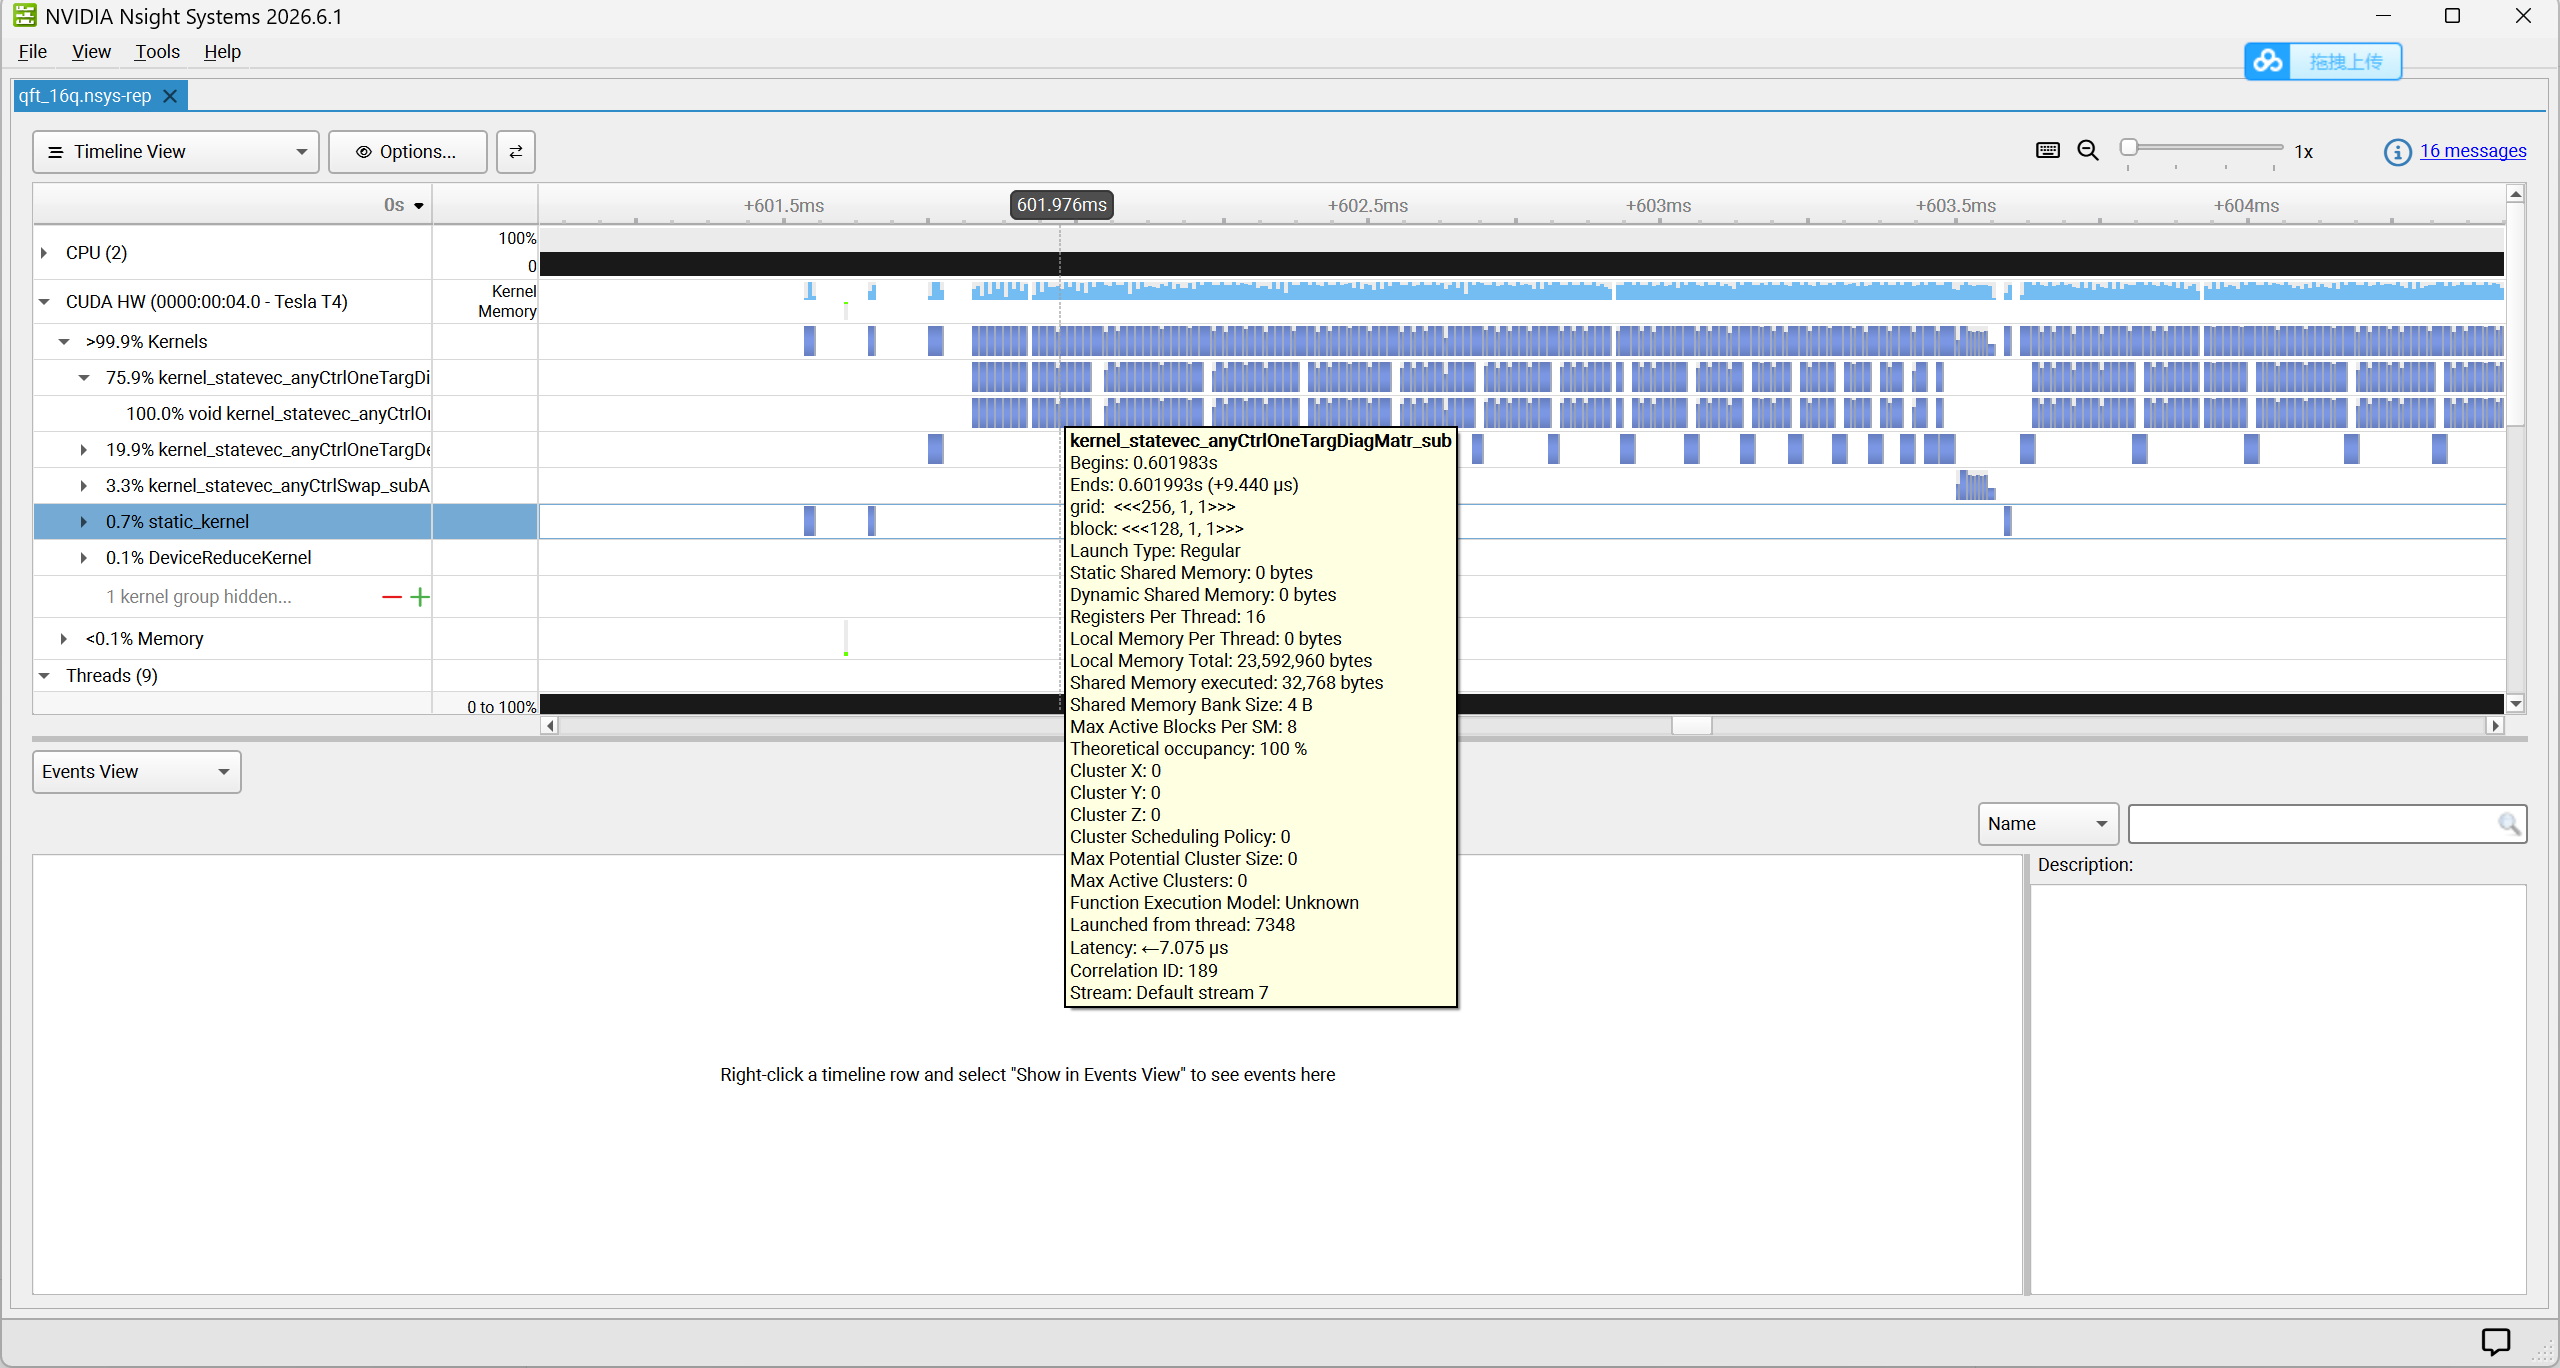
\includegraphics[width=\textwidth]{Q3/assets/image2.png}
\caption{Nsight Systems timeline at 16 qubits. The tooltip shows one phase kernel lasting 9.440 \(\mu\)s.}
\end{figure}

\begin{figure}[H]
\centering
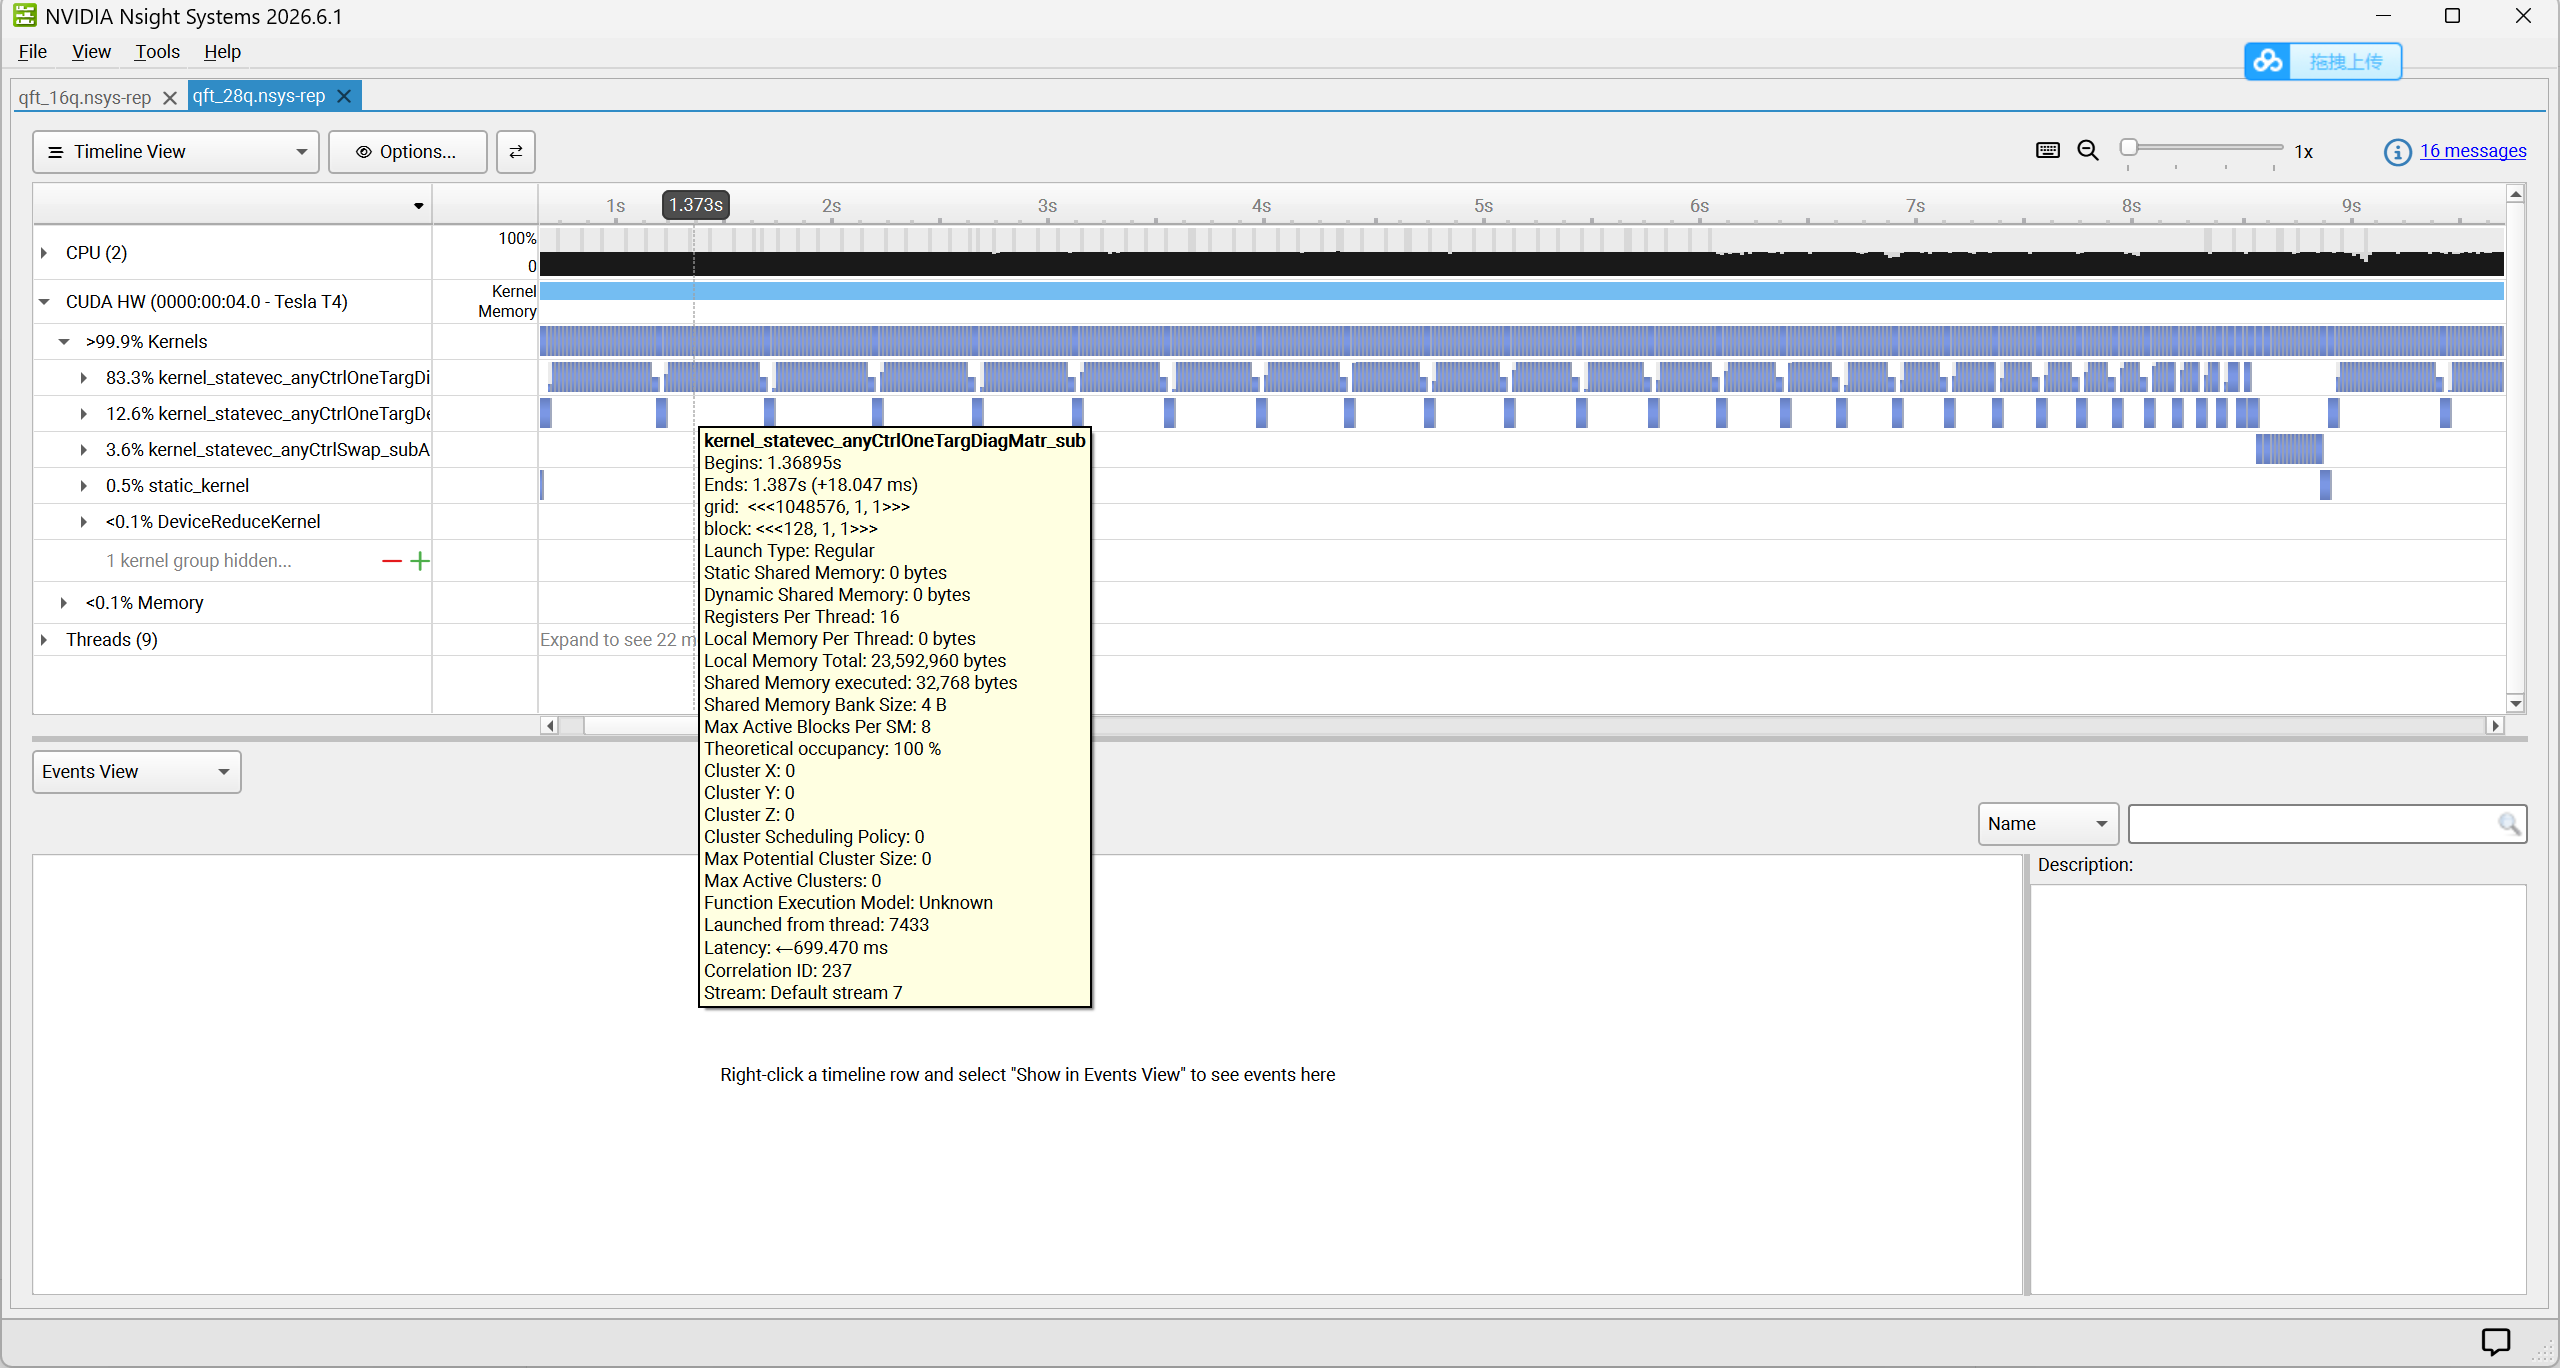
\includegraphics[width=\textwidth]{Q3/assets/image3.png}
\caption{Nsight Systems timeline at 28 qubits. The tooltip shows the same phase kernel lasting 18.047 ms.}
\end{figure}

\end{document}
